%!TEX root = spores.tex

\section{\Sphinxes: the Sphinx header format Extended for Sets of nodes}%
\label{Sphinxes}

\Textcite{Sphinx} designed \iac{UC} secure message format for mixes, called 
Sphinx.
Since it is \ac{UC} secure, it provably implements an ideal onion routing 
functionality.
\Ie, it provides bitwise unlinkability on the forward route, hides the path 
length, makes replies indistinguishable from forward messages and resists 
tagging attacks.
It is also compact with only 224 bytes of header for a five-hop path with 
128-bit security. \sonja{what about the CL properties?}
Sphinx only provides one node per onion layer; in this section we extend Sphinx 
to \Sphinxes, which allows for multiple nodes per onion layer.
(See \cref{fig:OR-POR}.)
% AL: Bounded random-walk....
As such, \Sphinxes could be described as a bounded random-walk protocol, \ie the 
each node selects the next node from a set restricted by the source.

\begin{figure}
  \centering
  %  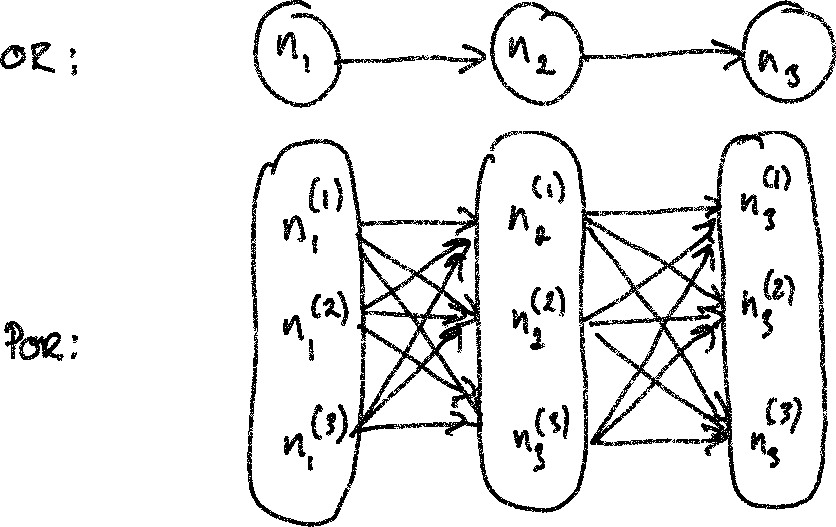
\includegraphics[width=\linewidth]{figures/OR-POR.png}
    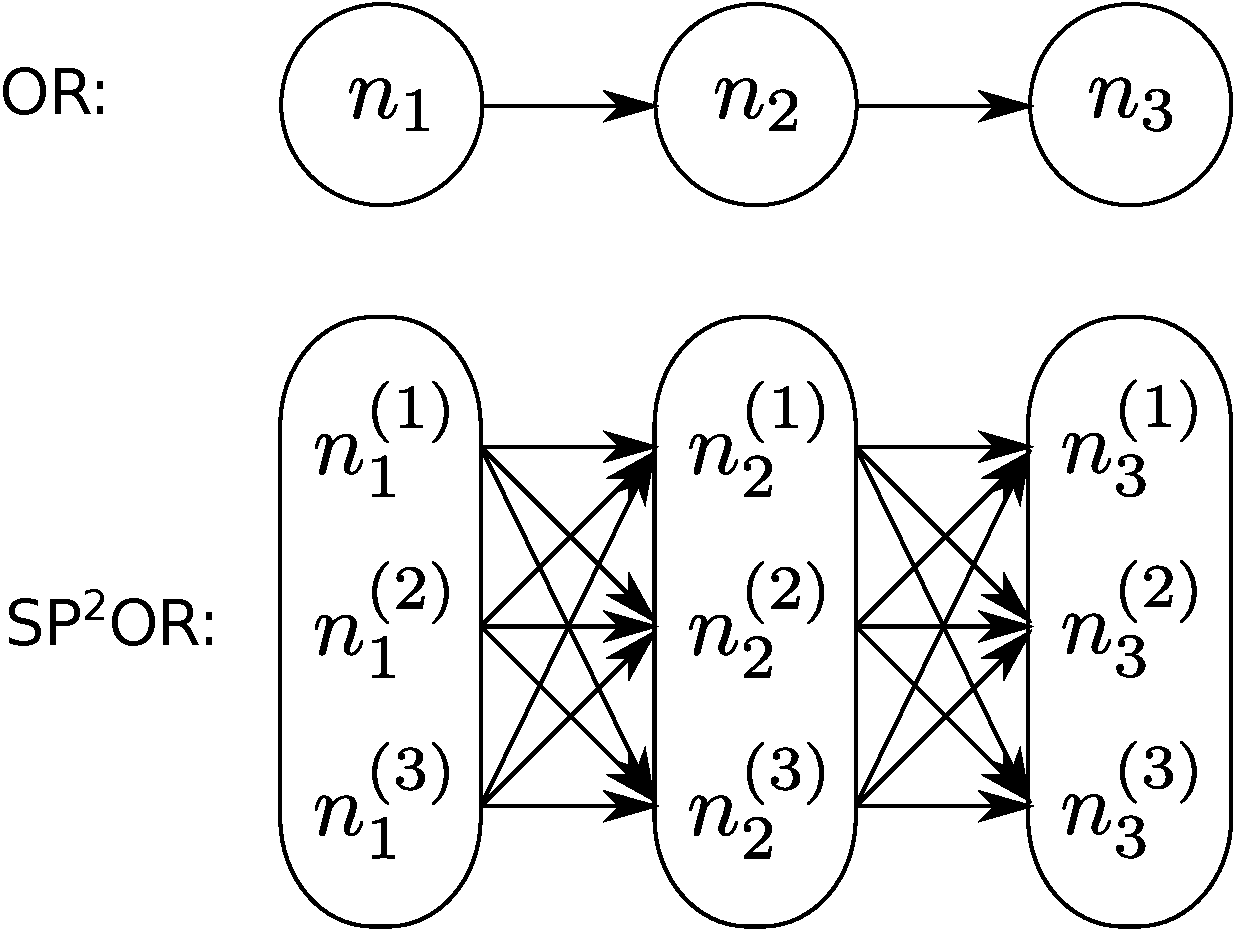
\includegraphics[width=0.65\linewidth]{figures/principle_SPOR.pdf}
  \caption{\label{fig:OR-POR}%
    Illustration of the conceptual difference between traditional onion routing 
and mixing (OR, top) and \ac{SPOR} (bottom).
    %\commentDaniel{This figure should be fixed, issue \#42.}
  }
\end{figure}

\subsubsection{Overview of the Sphinx header format}

We will now give an overview of the Sphinx header format.
The idea is not to give a detailed description of Sphinx, but to give the 
reader enough understanding of Sphinx to understand the changes we make to 
achieve \Sphinxes.
For a more detailed understanding of Sphinx, we refer the reader to the 
description in the original Sphinx paper~\cite{Sphinx}.

Each node \(n\) in the system has a long-term public-key pair: private key 
\(\sk_n\in \ZZ_q^*\) and public key \(\pk_n = g^{\sk_n}\in G\), where \(g\) 
generates a group \(G\) of prime order \(q\).

The Sphinx header (for the first node) is a triple \((\alpha_1, \beta_1, 
  \gamma_1)\), where \(\alpha_1\) is \iac{DHKE} exponent (\(g^x\), where \(x\) 
is a short-term secret chosen randomly for each header), \(\beta_1\) is the 
encrypted routing data and \(\gamma_1\) is \iac{MAC} for \(\beta_1\).
The payload data, \(\delta\), is treated separately from the header.

The first node in the path, with keys \((\pk_1, \sk_1)\), will compute the 
shared secret \(s_1 = \alpha_1^{\sk_1}\), \ie complete the \ac{DHKE} round.
Since \(\pk_1\) is an authenticated key, the sender can be sure that only this 
particular node can process the first layer of the onion.

The shared secret \(s_1\) is then used to derive various keys.
One of them is the key for the \ac{MAC} (\(\gamma_1\)) to verify the integrity 
of the header (\(\beta_1\)).
If \(\beta_1\) is correct, another key is derived from \(s_1\) to decrypt 
\(\beta_1\) to get \(d_2\concat \gamma_2\concat \beta_2\), where \(d_2\) is the 
address of the second node in the path.

We note that \(\beta_i\) is encrypted using a stream cipher.
Thus we can append zeros before decryption to keep the ciphertext length 
constant.
Since we append \emph{before} decryption, those appended zeros will look 
completely random to the next node, thus the position on the path is hidden.

Finally, \(\alpha_1\) is blinded into \(\alpha_2\) with a key derived from 
\(s_1\).
Then the triple \((\alpha_2, \beta_2, \gamma_2)\) is sent to the node with 
address \(d_2\). When node \(n\) discovers \(d_{n+1} = *\) it knows that the message is intended 
for itself and thus stops the forwarding.

\subsubsection{The \Sphinxes extension for sets of nodes}

We will now extend Sphinx to do \ac{SPOR}: instead of providing only \(d_{i+1}\) 
in \(\beta_i\), we will have a set \(\{d_{i+1}^{(1)}, \dotsc, d_{i+1}^{(m)}\}\) 
of \(m\) alternative next nodes.
This means that all \(m\) nodes must be able to compute the same shared secret 
\(s_{i+1}\).
We do this by adding one layer of indirection.

In Sphinx, the public key for layer \(i\) is denoted as \(\pk_i\).
Since we have \(m\) alternative nodes with different keys, let us denote them 
by \(\pk_i^{(1)}, \dotsc, \pk_i^{(m)}\).

We extend the header to a quadruple \((\alpha_i, C_i, \beta_i, \gamma_i)\), 
where \(\alpha_i, \beta_i, \gamma_i\) are the same as before.
We let the shared secret \(s_i\) be chosen uniformly randomly instead of being 
computed as \(\alpha_i^{\sk_i}\).
We now compute one shared secret per alternative node, \ie \(s_i^{(j)} = 
  \alpha_i^{\sk_i^{(j)}}\) for \(1\leq j\leq m\).
Then \(C_i = c_i^{(1)}\concat \dotsb\concat c_i^{(m)}\) is the concatenation of 
ciphertexts \(c_i^{(j)} = \Enc[_{s_i^{(j)}}][s_i]\), where \(\Enc\) is 
\iac{SKE} algorithm and each ciphertext contains the shared secret \(s_i\) 
encrypted under the individual keys \(s_i^{(j)}\). 

When a node receives this new header, it will compute \(s_i^{(j)}\gets 
  \alpha_i^{\sk_i^{(j)}}\).
Then, it will try to decrypt each ciphertext component \(c_i^{(k)}\) of \(C_i\) 
to get \(\hat s_i\).
If \iac{MAC} key that successfully verifies \(\beta_i\) using \(\gamma_i\) can 
be derived from \(\hat s_i\), then the node knows that \(\hat s_i = s_i\).


\subsubsection{\Sphinxes algorithms and \acf*{SPOR}}

\Sphinxes provides the following algorithms:
\begin{itemize}
  \item \(\CreateHeader\) creates a header.

  \item \(\CreateFwd\) constructs a header to be used for forward messages.

  \item \(\CreateReply\) constructs a header to be used for replies.

  \item \(\UseReply\) takes a reply header and attaches a message.

  \item \(\ProcessHeader\) is the algorithm for processing incoming messages.
\end{itemize}

We will synchronize our detailed descriptions with that of 
Sphinx~\cite{Sphinx}, hence we will use the following notation:
\begin{itemize}
  \item \(\kappa\) is the security parameter.
    The adversary must thus do about \(2^\kappa\) work to break the security.

  \item \(r\) is the maximum number of layers (hops, nodes) that a message will 
    traverse before reaching its destination.
  % I spent minutes looking for w_L: it deserves its bullet!
  \item \(w_L\) is the maximum width of a layer, \ie the maximum 
    number of alternative nodes on a layer.

  \item \(\G\) is a prime-order cyclic group satisfying the \ac{DH} assumption.

  \item \(\mac\colon \bin^\kappa\times \bin^*\to \bin^\kappa\) is \iac{MAC}.
    It can be instantiated as \eg SHA256-HMAC-128.

  \item \(\prg\colon \bin^\kappa\to \bin^{(2r+3)\kappa}\) is \iac{PRG}.
    It can be instantiated as any block cipher in counter mode.

  \item \(\prp\colon \bin^\kappa\times \bin^{l_\prp} \to \bin^{l_\prp}\) is 
    \iac{PRP} used to encrypt the payload data.
    \(l_\prp\) is the maximum length of the payload.
    (Shorter payloads are assumed to be properly padded.)

  \item \(\prp'\colon \bin^\kappa\times \bin^\kappa\times \bin^\kappa\) is 
    another \ac{PRP}.
    It is used to encapsulate keys.

  \item \(\hash_\mac, \hash_\prg, \hash_\prp. \hash_{\prp'}\) are all distinct 
    hash functions of the form \(\bin^\kappa\to \bin^\kappa\).
    They are used as key-derivation functions.

  \item \(\hash_\tau\colon \G^*\to \bin^{2\kappa}\) is used to identify 
    previously seen elements of \(\G^*\).

  \item \(\hash_\blind\colon \G^*\times \G^*\to \ZZ_q^*\) is used to compute 
    blinding factors.
    All the hash functions can be instantiated with truncated versions of hash 
    functions from the SHA-2 and -3 families.

  \item \(\N\subset \bin^\kappa\) is a set of node identifiers.
    Each node \(n\in \N\) has a private key \(\sk_n\in \ZZ_q^*\) and a public 
    key \(\pk_n = g^{\sk_n}\in \G^*\).
    We assume that the identifier--public-key pairs, \((n, \pk_n)\), are 
    distributed.
    (Sphinx made a difference between nodes and destinations, \ie the set 
    \(\D\) such that \(\D\cap \N = \emptyset\) and \(\D\cup \N\) is prefix 
    free, see~\cite{Sphinx} for details.
    We could do the same adoption, but we do not need that for the purposes of 
    this paper.)
    We have two special node identifiers:
    \(\nullnode\in \N\) is the null-node identifier, indicating an empty 
    address.
    \(\rdvnode\in \N\) is the crossover-node identifier, indicating that the 
    current node is the node at the end of one leg of a route that needs to cross
   over to another, and that the payload is \iac{SPOR} route 
    for forwarding.

  \item \(0_x\) denotes \(x\) zeroes.
    \(s_{[a..b]}\) denotes all bits from the \(a\)th bit to the \(b\)th of the 
    bit string \(s\).
\end{itemize}

We keep the nomenclature of mix headers and messages from Sphinx for
clarity but later apply them to onions and file chunks, repectively.

\paragraph*{The \(\CreateHeader\) algorithm}

This algorithm creates a header for \iac{SPOR}.
It is identical to that of Sphinx~\cite[\S 3.2]{Sphinx} except that we use a 
set of addresses and keys for each layer instead of only one address and key.
Also, we do not distinguish between addresses of destinations and routers.

The algorithm takes as input a unique identifier \(I\in \bin^\kappa\) and a set 
of layers \(L = \{L_0, \dotsc, L_\nu\}\) such that \(\nu+1\leq r\).
The last layer, \(L_\nu\), should be either \(\{\nullnode\}\) or 
\(\{\rdvnode\}\) to terminate the routing. \sonja{define v(nu)}

Remember that \(w_L\) is the maximum width of a layer, \ie the number of 
alternative nodes in the layer.
We let \(w_H = 2w_L+1\) be the header width:
each layer must accommodate the layer nodes' ciphertexts and addresses, \ie  
\(2w_L\) elements of \(\kappa\) bits,
and the \ac{MAC}, \ie one element of \(\kappa\) bits.

First we generate all the needed keys.
We compute \(\nu+1\) tuples:
\begin{align*}
  \alpha_0 &\gets g^\sk,
  & \secret_0 &\gets \bin^\kappa,
  & \blind_0 &\gets \hash_\blind(\alpha_0, \secret_0) \\
  \alpha_1 &\gets g^{\sk\blind_0},
  & \secret_1 &\gets \bin^\kappa,
  & \blind_1 &\gets \hash_\blind(\alpha_1, \secret_1) \\
  &\vdots &&\vdots && \vdots \\
  \alpha_\nu &\gets g^{\sk \blind_0\dotsb \blind_{\nu-1}},
  & \secret_\nu &\gets \bin^\kappa,
  & \blind_\nu &\gets \hash_\blind(\alpha_\nu, s_\nu).
\end{align*}
In addition, we compute:
\begin{align*}
  \secret_0^{(0)} &\gets \pk_{n_0^{(0)}}^\sk,
  & \dotsc, &
  & \secret_0^{(|L_0|-1)} &\gets \pk_{n_0^{(|L_0|-1)}}^\sk \\
  \secret_1^{(0)} &\gets \pk_{n_1^{(0)}}^{\sk \blind_0},
  & \dotsc, &
  & \secret_1^{(|L_1|-1)} &\gets \pk_{n_1^{(|L_1|-1)}}^{\sk \blind_0} \\
  & \vdots &&& \vdots \\
  \secret_\nu^{(0)} &\gets \pk_{n_\nu^{(0)}}^{\sk \blind_0\dotsb 
    \blind_{\nu-1}},
  & \dotsc, &
  & \secret_\nu^{(|L_\nu|-1)} &\gets \pk_{n_\nu^{(|L_\nu|-1)}}^{\sk 
    \blind_0\dotsb \blind_{\nu-1}}.
\end{align*}
We note that a node \(n_i^{(j)}\) can compute \(s_i^{(j)}\) since \[
  s_i^{(j)} = \pk_{n_i^{(j)}}^{\sk \blind_0\dotsb \blind_{i-1}} = 
  \alpha_i^{\sk_{n_i^{(j)}}}.
\]
We then construct the ciphertexts:
\begin{align*}
  C_0 &= \prp'\left(\hash_{\prp'}\left(s_0^{(0)}\right), s_0\right)
  \concat \dotsb
  \concat \prp'\left(\hash_{\prp'}\left(s_0^{(|L_0|-1)}\right), s_0\right) \\
  C_1 &= \prp'\left(\hash_{\prp'}\left(s_1^{(0)}\right), s_1\right)
  \concat \dotsb
  \concat \prp'\left(\hash_{\prp'}\left(s_1^{(|L_1|-1)}\right), s_1\right) \\
  & \vdots \\
  C_\nu &= \prp'\left(\hash_{\prp'}\left(s_\nu^{(0)}\right), s_\nu\right)
  \concat \dotsb
  \concat \prp'\left(\hash_{\prp'}\left(s_\nu^{(|L_\nu|-1)}\right) 
    s_\nu\right),
\end{align*}
and pad them to \(w_L\kappa\) bits with uniformly random bits.

Next we need to compute the padding \(\phi_i\) for each layer \(i\).
We must do this to predict the padding introduced at each layer so that we 
can compute the correct \acp{MAC} (\(\gamma_i\)).
The padding for the outermost layer (layer 0) is the empty string, thus \(\phi_0 
  \gets \epsilon\).
Then, for layers \(1\leq i\leq \nu\), we get
\begin{multline*}
  \phi_i\gets \left\{\phi_{i-1}\concat 0_{w_H\kappa}\right\}\oplus \\
  \left\{\prg\left(\hash_\prg\left(s_{i-1}\right)\right)_{[(w_H(r-i)+3)\kappa..(2r+3)\kappa-1]}\right\}.
\end{multline*}

Next we will use the above computations to arrive at the mix headers \(M_i = 
  (\alpha_i, \beta_i, \gamma_i)\).
\(\alpha_i\) was computed above, so we will compute \(\beta_i\) and 
\(\gamma_i\).
We must compute \(\beta_i\) in reverse order. \sonja{why? layering?}
We let \(\beta_{\nu} = I\concat 0_{(w_H r-1)\kappa}\), then, for \(\nu < i\leq 
  0\), we let
\begin{align*}
  \beta_i &\gets \left\{L_{i+1}\concat C_{i+1}\concat \gamma_{i+1}\concat 
    (\beta_{i+1})_{[0..(w_H r-1)\kappa-1]}\right\}, \\
  \gamma_i &\gets \mac\left( \hash_\mac\left(s_i\right), \beta_i \right).
\end{align*}

\paragraph*{The \(\CreateFwd\) algorithm}

This algorithm computes a forward header with a message to be delivered to the 
destination.
It takes as input a sequence, \(L = \{L_0, \dotsc, L_\nu\}\), of node sets, 
such that \(\nu+1\leq r\) and \(L_\nu\) is either \(\{\nullnode\}\) or 
\(\{\rdvnode\}\), and a message \(m\).
(\Ie \(L_{\nu-1}\) is the final destination.)

It first runs \(\CreateHeader\) with \(I = 0_\kappa\) to compute a mix header 
\(M_0\) and the keys \(s_i\) for each layer \(i\).
Then, for \(\nu\leq i\leq 0\), it will compute
\begin{equation*}
  \delta_i = \prp\left(
    \hash_\prp\left(s_i\right),
    \delta_{i+1}\right),
\end{equation*}
where \(\delta_{\nu+1}\) is the message \(m\).

\paragraph*{The \(\CreateReply\) algorithm}

This algorithm prepares a header that can be used for anonymous replies.
It takes as input a sequence, \(L = \{L_0, \dotsc, L_\nu\}\), of node sets, 
such that \(\nu+1\leq r\), \(L_\nu\) is either \(\{\nullnode\}\) or 
\(\{\rdvnode\}\) and \(L_{\nu-1}\) is the set of own addresses.

It first runs \(\CreateHeader\) with \(I\rgets \bin^\kappa\) to compute a mix 
header \(M_0\) and the keys \(s_i\) for each layer \(i\).
It chooses uniformly randomly a key \(\tilde k\rgets \bin^\kappa\).
Finally, it returns
\(I\),
the tuple of keys \((\tilde k, \hash_\prp(s_0), \dotsc, \hash_\prp(s_\nu))\),
and \((L_0, M_0, \tilde k)\).

The tuple of keys must be stored in a local table indexed by \(I\).
The tuple \((L_0, M_0, \tilde k)\) should be given to the sender who wants to 
use the anonymous reply.

\paragraph*{The \(\UseReply\) algorithm}

This algorithm takes a reply header \((L_0, M_0, \tilde k)\) and a message 
\(m\) as input.
It then returns \((M_0, \prp(\tilde k, m))\) which should be sent to any node 
in \(L_0\).

\paragraph*{The \(\ProcessHeader\) algorithm}

The algorithm takes as input a header \((M, \delta)\), where \(M = (\alpha, C, 
  \beta, \gamma)\in \G^*\times (\bin^\kappa)^{w_L} \times \bin^{(w_H 
    r+1)\kappa}\times bin^\kappa\times \bin^{l_\prp}\), and an auxiliary 
function \(\ProcessMessage\) which processes messages destined to itself.
Let \(\sk\) be the node's private key.

First, it computes the key \(s_i^{(j)}\gets \alpha^\sk\).
Then it trial-and-error decrypts every \(c_k\) in \(C = c_0\concat 
  \dotsb\concat c_{w_L-1}\) (\(0\leq k< w_L\)) to \(\hat s_i\gets \prp^{\prime 
    -1}\left(s_i^{(j)}, c_k\right)\).
If \(\gamma = \mac\left(\hat s_i, \beta\right)\), then \(\hat s_i = s_i\) is 
correct.
If the \ac{MAC} does not verify correctly for any key, then the algorithm 
aborts.

If the \ac{MAC} computed correctly, compute \(t\gets \hash_\tau(s_i)\).
If \(t\) is already in the table of seen (mix, not IP) packets, drop the packet.
Otherwise, add \(t\) to the table and decrypt \(\beta\):
\begin{equation*}
  L'\concat C'\concat \gamma'\concat \beta'\gets \{\beta\concat 0_{w_H 
    \kappa}\}
  \oplus \prg(\hash_\prg(s_i))
\end{equation*}

If \(L' = \{\nullnode\}\), the packet is addressed to the current node.
Parse the first \(\kappa\) bits of \(\beta'\) as an identifier \(I\).
Pass \((I, \delta)\) to the \(\ProcessMessage\) algorithm.

If \(L' = \{\rdvnode\}\), the packet payload contains another \Sphinxes packet 
to be forwarded.
Decrypt the payload \(\delta\) to get the mix packet \((M', \delta')\gets 
  \prp^{-1}(\hash_\prp(s_i), \delta)\).
Run the \(\ProcessHeader\) algorithm with \((M', \delta')\) and 
\(\ProcessMessage\) as input.

Otherwise. \(\beta'\) should be forwarded to \(L'\).
Compute the blinding factor \(b\gets \hash_\blind(\alpha, s_i)\) and let 
\(\alpha'\gets \alpha^b\).
Choose a node \(n\rgets L'\) uniformly at random.
Send \((\alpha', C', \beta', \gamma')\) to \(n\).
If sending to \(n\) fails, choose another node from \(L'\) uniformly at random.
If all nodes in \(L'\) fail, the algorithm drops the packet and fails silently.

